\chapter{Complete Link Budget Analysis}
\label{ch:link-budget}

\begin{nontechnical}
\textbf{Link budget is like a financial budget for radio power}---you start with transmit power, subtract losses, add gains, and see if there's enough ``money'' (signal) left at the receiver!

\textbf{The fundamental question:} ``If I transmit from HERE to THERE, will the receiver get enough signal?''

\textbf{The accounting:}

\textbf{START (Transmit power):}
\begin{itemize}
\item WiFi router: 100~mW (20~dBm)
\item Cell tower: 20~W (43~dBm)
\item Satellite: 100~W (50~dBm)
\end{itemize}

\textbf{GAINS (things that help):}
\begin{itemize}
\item \textbf{Transmit antenna gain:} Directional antenna focuses power
  \begin{itemize}
  \item WiFi router: $+2$~dB
  \item Satellite dish: $+40$~dB (very focused!)
  \end{itemize}
\item \textbf{Receive antenna gain:} Bigger antenna collects more
  \begin{itemize}
  \item Phone: $0$~dB (tiny antenna)
  \item Satellite dish: $+35$~dB
  \end{itemize}
\end{itemize}

\textbf{LOSSES (things that hurt):}
\begin{itemize}
\item \textbf{Free-space path loss:} Signal spreads with distance
  \begin{itemize}
  \item WiFi (50~m): $-74$~dB
  \item Cell tower (1~km): $-100$~dB
  \item Satellite (36,000~km): $-206$~dB!
  \end{itemize}
\item \textbf{Obstacles:} Walls, trees, rain
  \begin{itemize}
  \item One wall: $-5$~dB
  \item Heavy rain: $-10$~dB
  \end{itemize}
\item \textbf{Cable losses:} Connectors, cables ($-1$ to $-3$~dB)
\end{itemize}

\textbf{END (Received power):} Must be stronger than noise floor! Typical requirement: Signal $>$ Noise $+ 10$ to $20$~dB.

\textbf{Real example---WiFi link:} Transmit 20~dBm $+$ antenna 2~dB $= $ 22~dBm EIRP. Subtract free-space loss 74~dB and wall loss 10~dB $= -62$~dBm received. Noise floor $-90$~dBm gives SNR $= 28$~dB. Link works!

\textbf{Fun fact:} Voyager~1 spacecraft (over 13 billion miles away) transmits at 23~W. By the time it reaches Earth, the signal is $10^{-16}$~watts! Only massive 70-meter dishes with careful link budgets can hear it.
\end{nontechnical}

\section{Overview}

\textbf{Link budget} is a comprehensive accounting of \textbf{all gains and losses} from transmitter to receiver, determining whether a communication link will function reliably under specified conditions.

\begin{keyconcept}
Link budget analysis answers the critical question: \textbf{``Will the receiver obtain sufficient signal power to achieve the required data rate and bit error rate?''}
\end{keyconcept}

The fundamental link budget equation expresses received power in logarithmic units (dBm or dBW):
\begin{equation}
P_r = P_t + G_t - L_{\text{total}} + G_r
\label{eq:link-budget-basic}
\end{equation}
where:
\begin{itemize}
\item $P_r$ = received signal power (dBm)
\item $P_t$ = transmit power (dBm)
\item $G_t$ = transmit antenna gain (dBi)
\item $L_{\text{total}}$ = total path loss (dB)
\item $G_r$ = receive antenna gain (dBi)
\end{itemize}

\textbf{Link closure criterion:}
\begin{equation}
P_r > P_{\text{min}}
\label{eq:link-closure}
\end{equation}
where $P_{\text{min}}$ is the receiver sensitivity (minimum detectable signal).

\textbf{Link margin:}
\begin{equation}
M = P_r - P_{\text{min}} \quad \text{(dB)}
\label{eq:link-margin}
\end{equation}

The margin $M$ provides a safety buffer against fading, interference, and implementation losses. Positive margin is required for link closure; typical design targets range from 10 to 30~dB depending on the application.

\section{Link Budget System Overview}

A complete link budget encompasses transmitter, propagation path, and receiver subsystems. Figure~\ref{fig:link-budget-system} illustrates the end-to-end signal flow and associated gains and losses.

\begin{center}
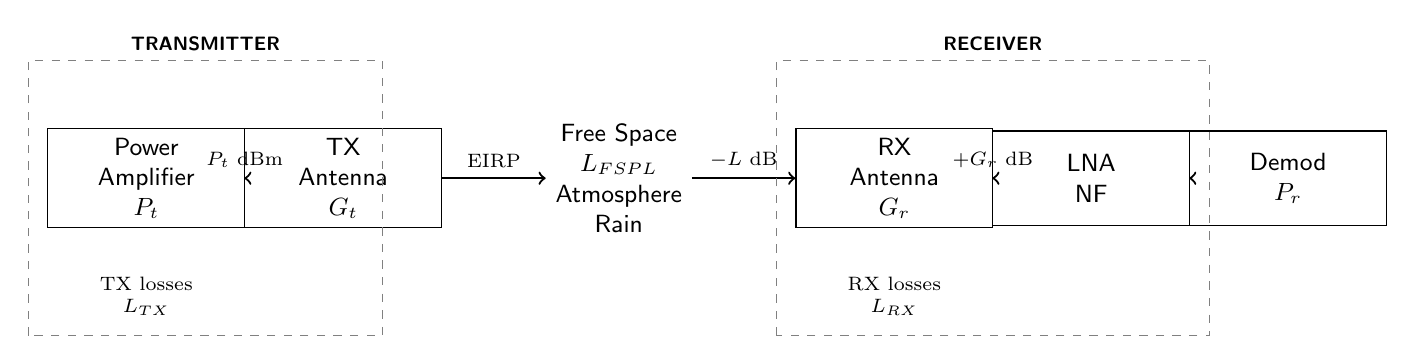
\begin{tikzpicture}[
  block/.style={rectangle, draw, minimum width=2.5cm, minimum height=1.2cm, font=\sffamily\small, align=center},
  gain/.style={isosceles triangle, draw, shape border rotate=0, minimum width=1cm, minimum height=1.2cm, font=\sffamily\scriptsize},
  node distance=1.8cm,
  font=\small
]
% Transmitter chain
\node[block] (pa) {Power\\Amplifier\\$P_t$};
\node[block, right of=pa, node distance=2.5cm] (txant) {TX\\Antenna\\$G_t$};

% Path
\node[right of=txant, node distance=3.5cm, align=center, font=\sffamily\small] (path) {Free Space\\$L_{\text{FSPL}}$\\Atmosphere\\Rain};

% Receiver chain
\node[block, right of=path, node distance=3.5cm] (rxant) {RX\\Antenna\\$G_r$};
\node[block, right of=rxant, node distance=2.5cm] (lna) {LNA\\NF};
\node[block, right of=lna, node distance=2.5cm] (demod) {Demod\\$P_r$};

% Signal flow
\draw[->,thick] (pa) -- node[above,font=\scriptsize] {$P_t$~dBm} (txant);
\draw[->,thick] (txant) -- node[above,font=\scriptsize] {EIRP} (path);
\draw[->,thick] (path) -- node[above,font=\scriptsize] {$-L$~dB} (rxant);
\draw[->,thick] (rxant) -- node[above,font=\scriptsize] {$+G_r$~dB} (lna);
\draw[->,thick] (lna) -- (demod);

% Loss/gain annotations
\node[below of=pa, node distance=1.5cm, font=\scriptsize, align=center] {TX losses\\$L_{\text{TX}}$};
\node[below of=rxant, node distance=1.5cm, font=\scriptsize, align=center] {RX losses\\$L_{\text{RX}}$};

% System boundaries
\draw[dashed, gray] (-1.5,-2) rectangle (3,1.5);
\node[above, font=\sffamily\scriptsize\bfseries] at (0.75,1.5) {TRANSMITTER};

\draw[dashed, gray] (8,-2) rectangle (13.5,1.5);
\node[above, font=\sffamily\scriptsize\bfseries] at (10.75,1.5) {RECEIVER};
\end{tikzpicture}
\end{center}

\section{Link Budget Components}\label{link-budget-components}

\subsection{Transmitter Side}

\subsubsection{Transmitted Power}

The transmitted power $P_t$ is the RF power delivered to the transmit antenna after accounting for all losses in the transmitter chain:
\begin{equation}
P_t = P_{\text{amp}} - L_{\text{TX}}
\label{eq:tx-power}
\end{equation}
where:
\begin{itemize}
\item $P_{\text{amp}}$ = power amplifier output power (dBm)
\item $L_{\text{TX}}$ = transmitter losses including cables, filters, circulators, and connectors (dB)
\end{itemize}

\begin{calloutbox}{Example: WiFi Router Transmit Power}
\textbf{Given:}
\begin{itemize}
\item PA output: $P_{\text{amp}} = 20$~dBm (100~mW)
\item Cable/connector loss: $L_{\text{TX}} = 0.5$~dB
\end{itemize}

\textbf{Solution:}
\begin{equation*}
P_t = 20 - 0.5 = 19.5\text{~dBm}
\end{equation*}
\end{calloutbox}

\subsubsection{Transmit Antenna Gain and EIRP}

The transmit antenna gain $G_t$ is measured relative to an isotropic radiator and expressed in dBi. The combination of transmit power and antenna gain yields the \textbf{Effective Isotropic Radiated Power (EIRP)}:
\begin{equation}
\text{EIRP} = P_t + G_t
\label{eq:eirp}
\end{equation}

\textbf{Example:} For $P_t = 19.5$~dBm and $G_t = 2$~dBi (omnidirectional WiFi antenna):
\begin{equation*}
\text{EIRP} = 19.5 + 2 = 21.5\text{~dBm}
\end{equation*}

\begin{warningbox}
\textbf{Regulatory compliance is mandatory.} Most jurisdictions limit EIRP to prevent interference. For example, FCC regulations limit EIRP to 36~dBm (4~W) for unlicensed 2.4~GHz WiFi operations. Exceeding these limits can result in legal penalties and harmful interference to other systems.
\end{warningbox}

\subsection{Propagation Path}

\subsubsection{Free-Space Path Loss}

Free-space path loss (FSPL) quantifies the attenuation of electromagnetic waves propagating through free space due to spherical wavefront expansion. The loss is derived from the Friis transmission equation:
\begin{equation}
L_{\text{FSPL}} = 20\log_{10}(d) + 20\log_{10}(f) + 20\log_{10}\left(\frac{4\pi}{c}\right)
\label{eq:fspl-full}
\end{equation}
where:
\begin{itemize}
\item $d$ = distance between transmitter and receiver (m)
\item $f$ = frequency (Hz)
\item $c = 3 \times 10^8$~m/s = speed of light
\end{itemize}

\textbf{Practical form} with distance in kilometers and frequency in MHz:
\begin{equation}
L_{\text{FSPL}} = 32.45 + 20\log_{10}(d_{\text{km}}) + 20\log_{10}(f_{\text{MHz}})
\label{eq:fspl-practical}
\end{equation}

\begin{calloutbox}{Example: WiFi Free-Space Path Loss}
\textbf{Given:}
\begin{itemize}
\item Frequency: $f = 2.4$~GHz $= 2400$~MHz
\item Distance: $d = 100$~m $= 0.1$~km
\end{itemize}

\textbf{Solution:}
\begin{align*}
L_{\text{FSPL}} &= 32.45 + 20\log_{10}(0.1) + 20\log_{10}(2400) \\
&= 32.45 - 20 + 67.6 \\
&= 80.0\text{~dB}
\end{align*}
\end{calloutbox}

\textbf{Cross-reference:} See Chapter~\ref{ch:fspl} for detailed derivation and frequency dependence analysis.

\subsubsection{Atmospheric Absorption}

Oxygen and water vapor molecules exhibit resonant absorption at specific frequencies, producing additional attenuation. This effect becomes significant above 10~GHz and must be accounted for in satellite and millimeter-wave links.

\textbf{Zenith attenuation at sea level:}

\begin{center}
\begin{tabular}{@{}lll@{}}
\toprule
Frequency & Attenuation (dB/km) & Notes \\
\midrule
$< 10$~GHz & $< 0.01$ & Negligible \\
22.2~GHz & 0.2 & H$_2$O resonance \\
60~GHz & 15 & O$_2$ resonance (peak) \\
120~GHz & 2 & Secondary O$_2$ line \\
183~GHz & 5 & H$_2$O line \\
\bottomrule
\end{tabular}
\end{center}

\begin{calloutbox}{Example: Ka-band Satellite Atmospheric Loss}
\textbf{Given:}
\begin{itemize}
\item Frequency: 20~GHz
\item Elevation angle: $5°$ (path length $\approx 11$~km through atmosphere)
\item Attenuation rate: $\approx 0.05$~dB/km
\end{itemize}

\textbf{Solution:}
\begin{equation*}
L_{\text{atm}} = 0.05 \times 11 = 0.55\text{~dB}
\end{equation*}
\end{calloutbox}

\subsubsection{Rain Attenuation}

Rain attenuation is the dominant propagation impairment for satellite links operating in Ku-band (12--18~GHz), Ka-band (26.5--40~GHz), and V-band (40--75~GHz). The \textbf{ITU-R rain attenuation model} expresses specific attenuation as:
\begin{equation}
\gamma_R = k \cdot R^{\alpha} \quad \text{(dB/km)}
\label{eq:rain-attenuation}
\end{equation}
where:
\begin{itemize}
\item $\gamma_R$ = specific rain attenuation (dB/km)
\item $R$ = rain rate (mm/hr)
\item $k, \alpha$ = frequency-dependent coefficients (from ITU-R tables)
\end{itemize}

\begin{calloutbox}{Example: Ku-band Heavy Rain Attenuation}
\textbf{Given:}
\begin{itemize}
\item Frequency: 12~GHz (Ku-band downlink)
\item Rain rate: $R = 25$~mm/hr (heavy rain)
\item Path length through rain: 4~km
\item ITU-R coefficients: $k = 0.0188$, $\alpha = 1.217$
\end{itemize}

\textbf{Solution:}
\begin{align*}
\gamma_R &= 0.0188 \times 25^{1.217} = 1.2\text{~dB/km} \\
L_{\text{rain}} &= 1.2 \times 4 = 4.8\text{~dB}
\end{align*}
\end{calloutbox}

\textbf{Design criterion:} For 99\% link availability, design for the rain rate exceeded 1\% of the time. Typical values: temperate climate 12~mm/hr, tropical climate 42~mm/hr.

\subsubsection{Other Propagation Effects}

Additional impairments must be considered depending on the link geometry, frequency band, and environmental conditions:

\begin{center}
\begin{tabular}{@{}p{0.25\linewidth}p{0.25\linewidth}p{0.40\linewidth}@{}}
\toprule
\textbf{Effect} & \textbf{Typical Loss} & \textbf{When Applicable} \\
\midrule
Ionospheric scintillation & 1--20~dB & L-band satellite, equatorial, solar max \\
Tropospheric scintillation & 0.5--2~dB & Low elevation, $> 10$~GHz \\
Polarization mismatch & 0--$\infty$~dB & Antenna misalignment, Faraday rotation \\
Multipath fading & 10--30~dB & Mobile, urban NLOS \\
Foliage loss & 0.3--1~dB/m & Trees, vegetation (VHF/UHF) \\
Building penetration & 5--20~dB & Indoor (depends on frequency, materials) \\
\bottomrule
\end{tabular}
\end{center}

\subsection{Receiver Side}

\subsubsection{Receive Antenna Gain}

The receive antenna gain $G_r$ follows the same definition as transmit antenna gain due to antenna reciprocity. Common antenna gains:

\begin{itemize}
\item \textbf{Omnidirectional:} $G_r = 0$~dBi (WiFi laptop, smartphone)
\item \textbf{Yagi antenna:} $G_r = 10$--15~dBi (TV reception, point-to-point)
\item \textbf{Parabolic dish:} $G_r = 30$--60~dBi (satellite ground stations)
\end{itemize}

\subsubsection{Receiver Losses}

Losses between the antenna and receiver input degrade the received signal:

\begin{itemize}
\item \textbf{Cable loss:} 0.5--3~dB (depends on length, frequency, cable type)
\item \textbf{Connector loss:} 0.1--0.5~dB per connector
\item \textbf{Filter loss:} 0.5--2~dB (bandpass filters)
\item \textbf{Circulator/duplexer loss:} 0.5--1~dB
\end{itemize}

\begin{calloutbox}{Example: Satellite Ground Station Receiver Chain}
\textbf{Given:}
\begin{itemize}
\item Cable loss (dish to equipment room): 2~dB
\item Connector losses: 0.3~dB
\item LNA gain (at antenna): $-40$~dB (gain, not loss)
\end{itemize}

\textbf{Net effect:}
\begin{equation*}
L_{\text{net}} = 2 + 0.3 - 40 = -37.7\text{~dB (net gain)}
\end{equation*}

\textbf{Note:} Placing the LNA at the antenna minimizes cable losses before amplification, optimizing noise figure.
\end{calloutbox}

\subsubsection{Receiver Sensitivity}

Receiver sensitivity $P_{\text{min}}$ is the minimum signal power required to achieve a specified bit error rate (BER) or signal quality. It is computed from the thermal noise floor, receiver noise figure, required SNR, and implementation losses:
\begin{equation}
P_{\text{min}} = -174 + 10\log_{10}(B) + \text{NF} + \text{SNR}_{\text{req}} + L_{\text{impl}}
\label{eq:receiver-sensitivity}
\end{equation}
where:
\begin{itemize}
\item $-174$~dBm/Hz = thermal noise floor at $T = 290$~K
\item $B$ = receiver bandwidth (Hz)
\item $\text{NF}$ = receiver noise figure (dB)
\item $\text{SNR}_{\text{req}}$ = required SNR for target BER (dB)
\item $L_{\text{impl}}$ = implementation losses (quantization, imperfect synchronization, etc.) $\approx 1$--3~dB
\end{itemize}

\begin{calloutbox}{Example: WiFi 802.11n Receiver Sensitivity}
\textbf{Given:}
\begin{itemize}
\item Bandwidth: $B = 20$~MHz $= 73$~dBHz
\item Noise figure: $\text{NF} = 6$~dB (typical WiFi chipset)
\item Required SNR: $\text{SNR}_{\text{req}} = 5$~dB (QPSK 1/2 with FEC)
\item Implementation loss: $L_{\text{impl}} = 2$~dB
\end{itemize}

\textbf{Solution:}
\begin{align*}
P_{\text{min}} &= -174 + 73 + 6 + 5 + 2 \\
&= -88\text{~dBm}
\end{align*}
\end{calloutbox}

\section{Complete Link Budget Equation}

The complete link budget equation aggregates all transmitter gains, propagation losses, and receiver gains/losses:
\begin{equation}
P_r = \text{EIRP} - L_{\text{FSPL}} - L_{\text{atm}} - L_{\text{rain}} - L_{\text{other}} + G_r - L_{\text{RX}}
\label{eq:link-budget-complete}
\end{equation}

\textbf{Expanded form:}
\begin{equation}
P_r = [P_t + G_t] - L_{\text{FSPL}} - L_{\text{atm}} - L_{\text{rain}} - L_{\text{multipath}} - L_{\text{misc}} + [G_r - L_{\text{cable}}]
\label{eq:link-budget-expanded}
\end{equation}

\subsection{Link Margin}

Link margin quantifies the excess signal power available beyond the minimum required for operation:
\begin{equation}
M = P_r - P_{\text{min}}
\label{eq:margin-definition}
\end{equation}

\begin{keyconcept}
\textbf{Design guideline:} $M \geq 10$~dB provides adequate margin against fading, interference, and component aging. Systems with $M < 5$~dB are considered marginal and prone to outages.
\end{keyconcept}

Figure~\ref{fig:link-margin} illustrates the relationship between received power, sensitivity, and margin.

\begin{center}
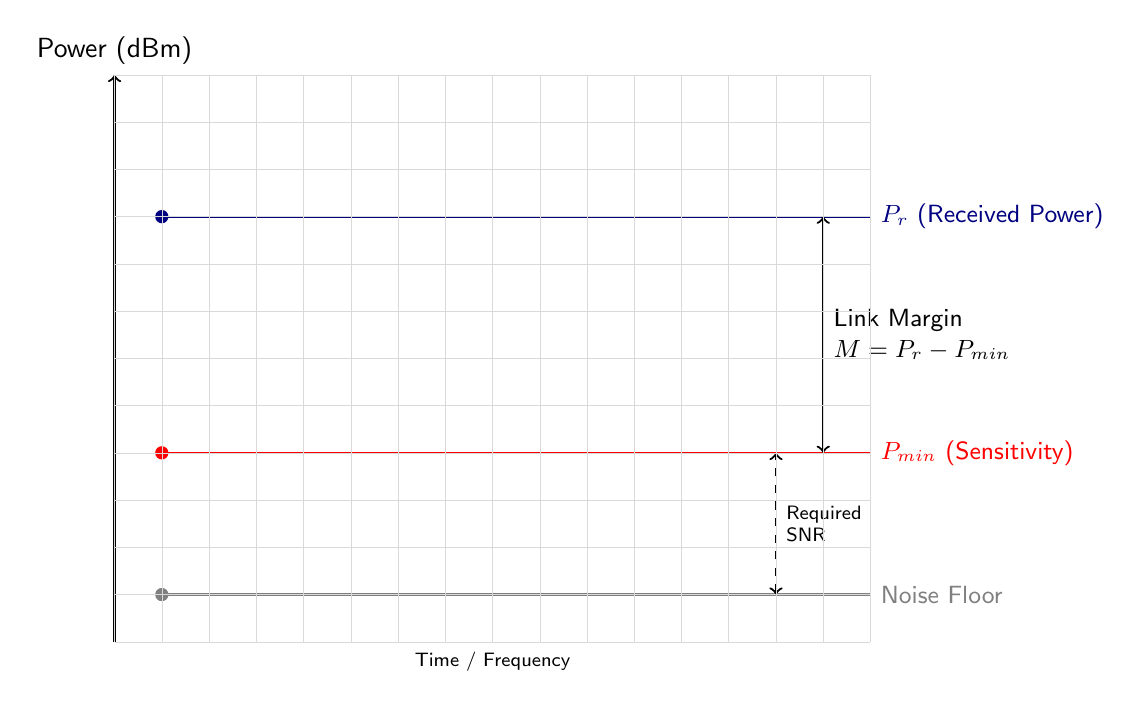
\begin{tikzpicture}[scale=1.2]
% Power levels
\draw[thick,->] (0,0) -- (0,6) node[above] {\sffamily Power (dBm)};

% Received power
\draw[thick, NavyBlue] (0.5,4.5) -- (8,4.5) node[right, font=\sffamily\small] {$P_r$ (Received Power)};
\fill[NavyBlue] (0.5,4.5) circle (2pt);

% Receiver sensitivity
\draw[thick, red] (0.5,2) -- (8,2) node[right, font=\sffamily\small] {$P_{\text{min}}$ (Sensitivity)};
\fill[red] (0.5,2) circle (2pt);

% Noise floor
\draw[thick, gray] (0.5,0.5) -- (8,0.5) node[right, font=\sffamily\small] {Noise Floor};
\fill[gray] (0.5,0.5) circle (2pt);

% Margin annotation
\draw[<->, thick] (7.5,2) -- (7.5,4.5) node[midway, right, align=left, font=\sffamily\small] {Link Margin\\$M = P_r - P_{\text{min}}$};

% Required SNR annotation
\draw[<->, thick, dashed] (7,0.5) -- (7,2) node[midway, right, align=left, font=\sffamily\scriptsize] {Required\\SNR};

% Grid
\draw[very thin, gray!30] (0,0) grid[step=0.5] (8,6);

% Labels
\node[below, font=\sffamily\scriptsize] at (4,0) {Time / Frequency};
\end{tikzpicture}
\end{center}

\subsection{Example 1: WiFi Indoor
Link}\label{example-1-wifi-indoor-link}

\textbf{Scenario}: 2.4 GHz WiFi, 802.11n, 20 MHz, QPSK 1/2, 50 m indoor

\subsubsection{Transmitter}\label{transmitter}

\begin{itemize}
\tightlist
\item
  PA output: 20 dBm
\item
  Cable loss: 0.5 dB
\item
  \textbf{P\_t}: 19.5 dBm
\item
  Antenna gain: 2 dBi
\item
  \textbf{EIRP}: 21.5 dBm
\end{itemize}

\subsubsection{Path}\label{path}

\begin{itemize}
\tightlist
\item
  Free-space loss @ 50 m, 2.4 GHz:
\end{itemize}

\[
L_{\text{FSPL}} = 32.45 + 20\log_{10}(0.05) + 20\log_{10}(2400) = 32.45 - 26 + 67.6 = 74\ \text{dB}
\]

\begin{itemize}
\tightlist
\item
  Wall penetration (2 walls \$\textbackslash times\$ 5 dB): 10 dB
\item
  \textbf{Total path loss}: 74 + 10 = 84 dB
\end{itemize}

\subsubsection{Receiver}\label{receiver}

\begin{itemize}
\tightlist
\item
  Antenna gain: 0 dBi (laptop internal)
\item
  Cable loss: 0 dB (integrated)
\item
  \textbf{Received power}:
\end{itemize}

\[
P_r = 21.5 - 84 + 0 = -62.5\ \text{dBm}
\]

\subsubsection{Sensitivity}\label{sensitivity}

\begin{itemize}
\tightlist
\item
  Thermal noise: -174 dBm/Hz + 73 dBHz = -101 dBm
\item
  NF: 6 dB
\item
  SNR\_req: 5 dB (QPSK 1/2)
\item
  Impl loss: 2 dB
\item
  \textbf{P\_min}: -101 + 6 + 5 + 2 = -88 dBm
\end{itemize}

\subsubsection{Margin}\label{margin}

\[
M = -62.5 - (-88) = 25.5\ \text{dB}
\]

\textbf{Result}: Link \textbf{closes comfortably} with 25.5 dB margin
(can tolerate fading, interference)

\begin{center}\rule{0.5\linewidth}{0.5pt}\end{center}

\subsection{Example 2: GEO Satellite Ku-band
Downlink}\label{example-2-geo-satellite-ku-band-downlink}

\textbf{Scenario}: 12 GHz downlink, 36,000 km slant range, 1 m dish RX,
clear sky

\subsubsection{Transmitter (Satellite)}\label{transmitter-satellite}

\begin{itemize}
\tightlist
\item
  Satellite PA: 100 W = 50 dBm
\item
  TX antenna gain: 30 dBi (spot beam)
\item
  \textbf{EIRP}: 80 dBm = 80 dBW
\end{itemize}

\subsubsection{Path}\label{path-1}

\begin{itemize}
\tightlist
\item
  Distance: 36,000 km
\item
  Frequency: 12 GHz
\end{itemize}

\[
L_{\text{FSPL}} = 32.45 + 20\log_{10}(36,000) + 20\log_{10}(12,000)
\]

\[
= 32.45 + 91.1 + 81.6 = 205\ \text{dB}
\]

\begin{itemize}
\tightlist
\item
  Atmospheric absorption (5\$\^{}\textbackslash circ\$ elevation): 0.5
  dB
\item
  Clear-sky rain (0.01 mm/hr): 0.01 dB (negligible)
\item
  Ionospheric scintillation margin: 2 dB
\item
  \textbf{Total path loss}: 205 + 0.5 + 0 + 2 = 207.5 dB
\end{itemize}

\subsubsection{Receiver (Ground Station)}\label{receiver-ground-station}

\begin{itemize}
\tightlist
\item
  Dish diameter: 1 m
\item
  Antenna gain (eff 60\%):
\end{itemize}

\[
G_r = 10\log_{10}\left(0.6 \times \left(\frac{\pi \times 1}{0.025}\right)^2\right) = 10\log_{10}(0.6 \times 1580) = 37.8\ \text{dBi}
\]

\begin{itemize}
\tightlist
\item
  LNA noise figure: 0.8 dB (cryogenic)
\item
  Cable loss: 1 dB
\item
  \textbf{Net RX gain}: 37.8 - 1 = 36.8 dB
\end{itemize}

\textbf{Received power}:

\[
P_r = 80 - 207.5 + 36.8 = -90.7\ \text{dBm}
\]

\subsubsection{Sensitivity (DVB-S2, QPSK 3/4, 36 MHz
bandwidth)}\label{sensitivity-dvb-s2-qpsk-34-36-mhz-bandwidth}

\begin{itemize}
\tightlist
\item
  Bandwidth: 36 MHz = 75.6 dBHz
\item
  Thermal noise: -174 + 75.6 = -98.4 dBm
\item
  NF: 0.8 dB (LNA at antenna)
\item
  SNR\_req: 6.5 dB (QPSK 3/4 with LDPC)
\item
  Impl loss: 1.5 dB
\item
  \textbf{P\_min}: -98.4 + 0.8 + 6.5 + 1.5 = -89.6 dBm
\end{itemize}

\subsubsection{Margin (Clear Sky)}\label{margin-clear-sky}

\[
M = -90.7 - (-89.6) = -1.1\ \text{dB}
\]

\textbf{Uh oh!} Link \textbf{fails} in clear sky (need higher gain or
more TX power)

\textbf{Fix}: Increase dish to 1.8 m - New gain: 37.8 + 20log(1.8) =
42.9 dBi - New \(P_r\): 80 - 207.5 + 42.9 = -84.6 dBm - \textbf{New
margin}: -84.6 - (-89.6) = \textbf{5 dB} (marginal)

\textbf{With 99\% rain margin} (add 5 dB rain attenuation): - \(P_r\) in
rain: -84.6 - 5 = -89.6 dBm - \textbf{Rain margin}: 0 dB (link at
threshold!)

\textbf{Better fix}: Use 2.4 m dish - Gain: 47.5 dBi - Clear sky: -80
dBm, margin 10 dB - 99\% rain: -85 dBm, margin 5 dB

\begin{center}\rule{0.5\linewidth}{0.5pt}\end{center}

\subsection{Example 3: Cellular LTE (2.6
GHz)}\label{example-3-cellular-lte-2.6-ghz}

\textbf{Scenario}: eNodeB to UE, 2.6 GHz, 10 MHz RB, QPSK 1/2, 5 km
suburban

\subsubsection{Transmitter (Cell Tower)}\label{transmitter-cell-tower}

\begin{itemize}
\tightlist
\item
  PA per antenna: 43 dBm (20 W)
\item
  TX antenna: 17 dBi (sector antenna)
\item
  Cable loss: 2 dB
\item
  \textbf{EIRP}: 43 + 17 - 2 = 58 dBm
\end{itemize}

\subsubsection{Path}\label{path-2}

\begin{itemize}
\tightlist
\item
  FSPL @ 5 km, 2.6 GHz:
\end{itemize}

\[
L_{\text{FSPL}} = 32.45 + 20\log_{10}(5) + 20\log_{10}(2600) = 32.45 + 14 + 68.3 = 115\ \text{dB}
\]

\begin{itemize}
\tightlist
\item
  Shadowing margin (suburban log-normal): 8 dB (for 90\% coverage)
\item
  Building penetration: 10 dB (indoor UE)
\item
  \textbf{Total path loss}: 115 + 8 + 10 = 133 dB
\end{itemize}

\subsubsection{Receiver (UE)}\label{receiver-ue}

\begin{itemize}
\tightlist
\item
  Antenna gain: -2 dBi (internal, near body)
\item
  \textbf{Received power}:
\end{itemize}

\[
P_r = 58 - 133 - 2 = -77\ \text{dBm}
\]

\subsubsection{Sensitivity (10 MHz, QPSK
1/2)}\label{sensitivity-10-mhz-qpsk-12}

\begin{itemize}
\tightlist
\item
  Bandwidth: 10 MHz = 70 dBHz
\item
  Thermal noise: -174 + 70 = -104 dBm
\item
  NF: 9 dB (smartphone front-end)
\item
  SNR\_req: 4 dB (QPSK 1/2 Turbo code)
\item
  Impl loss: 2 dB
\item
  \textbf{P\_min}: -104 + 9 + 4 + 2 = -89 dBm
\end{itemize}

\subsubsection{Margin}\label{margin-1}

\[
M = -77 - (-89) = 12\ \text{dB}
\]

\textbf{Result}: Link \textbf{closes} with 12 dB margin (adequate for
mobile fading)

\textbf{With Rayleigh fading} (10 dB fade depth @ 10\% time): - Faded
\(P_r\): -77 - 10 = -87 dBm - \textbf{Faded margin}: -87 - (-89) = 2 dB
(still works, but error rate increases)

\textbf{Diversity RX} (2 antennas, max ratio combining): - Diversity
gain: 5 dB (typical for 2-branch) - Effective \(P_r\) in fade: -87 + 5 =
-82 dBm - \textbf{Margin with diversity}: -82 - (-89) = 7 dB (much
better!)

\begin{center}\rule{0.5\linewidth}{0.5pt}\end{center}

\subsection{Link Budget Table
Template}\label{link-budget-table-template}

{\def\LTcaptype{} % do not increment counter
\begin{longtable}[]{@{}
  >{\raggedright\arraybackslash}p{(\linewidth - 8\tabcolsep) * \real{0.2750}}
  >{\raggedright\arraybackslash}p{(\linewidth - 8\tabcolsep) * \real{0.2000}}
  >{\raggedright\arraybackslash}p{(\linewidth - 8\tabcolsep) * \real{0.1750}}
  >{\raggedright\arraybackslash}p{(\linewidth - 8\tabcolsep) * \real{0.1750}}
  >{\raggedright\arraybackslash}p{(\linewidth - 8\tabcolsep) * \real{0.1750}}@{}}
\toprule\noalign{}
\begin{minipage}[b]{\linewidth}\raggedright
Parameter
\end{minipage} & \begin{minipage}[b]{\linewidth}\raggedright
Symbol
\end{minipage} & \begin{minipage}[b]{\linewidth}\raggedright
Value
\end{minipage} & \begin{minipage}[b]{\linewidth}\raggedright
Units
\end{minipage} & \begin{minipage}[b]{\linewidth}\raggedright
Notes
\end{minipage} \\
\midrule\noalign{}
\endhead
\bottomrule\noalign{}
\endlastfoot
\textbf{TRANSMITTER} & & & & \\
TX power (PA) & \(P_{\text{amp}}\) & & dBm & \\
TX losses & \(L_{\text{TX}}\) & & dB & Cables, filters \\
Transmit power & \(P_t\) & & dBm & \(P_{\text{amp}} - L_{\text{TX}}\) \\
TX antenna gain & \(G_t\) & & dBi & \\
\textbf{EIRP} & & & dBm & \(P_t + G_t\) \\
\textbf{PROPAGATION} & & & & \\
Distance & \(d\) & & km & \\
Frequency & \(f\) & & GHz & \\
Free-space loss & \(L_{\text{FSPL}}\) & & dB & 32.45 + 20log(d) +
20log(f) \\
Atmospheric loss & \(L_{\text{atm}}\) & & dB & \\
Rain attenuation & \(L_{\text{rain}}\) & & dB & ITU model \\
Other losses & \(L_{\text{other}}\) & & dB & Multipath, penetration,
etc. \\
\textbf{Total path loss} & \(L_{\text{total}}\) & & dB & Sum \\
\textbf{RECEIVER} & & & & \\
RX antenna gain & \(G_r\) & & dBi & \\
RX losses & \(L_{\text{RX}}\) & & dB & Cables, connectors \\
\textbf{Received power} & \(P_r\) & & dBm & EIRP - \(L_{\text{total}}\)
+ \(G_r\) - \(L_{\text{RX}}\) \\
\textbf{PERFORMANCE} & & & & \\
Bandwidth & \(B\) & & MHz & \\
Thermal noise & \(N_0\) & -174 + 10log(B) & dBm & \\
Noise figure & NF & & dB & \\
Noise power & \(N\) & \(N_0\) + NF & dBm & \\
Required SNR & SNR\_req & & dB & For target BER \\
Impl loss & \(L_{\text{impl}}\) & & dB & Typically 1-3 dB \\
\textbf{Sensitivity} & \(P_{\text{min}}\) & & dBm & \(N\) + SNR\_req +
\(L_{\text{impl}}\) \\
\textbf{MARGIN} & \(M\) & & dB & \(P_r - P_{\text{min}}\) \\
\end{longtable}
}

\begin{center}\rule{0.5\linewidth}{0.5pt}\end{center}

\subsection{Fade Margin Design
Guidelines}\label{fade-margin-design-guidelines}

\textbf{Clear-sky margin} (no fading): - \textbf{Satellite (GEO Ku/Ka)}:
5-10 dB - \textbf{Terrestrial LOS}: 10-15 dB - \textbf{Mobile (NLOS)}:
15-20 dB

\textbf{Rain margin} (satellite): - \textbf{Availability}: 99\%
\$\textbackslash rightarrow\$ 5-8 dB, 99.9\%
\$\textbackslash rightarrow\$ 10-15 dB, 99.99\%
\$\textbackslash rightarrow\$ 20-30 dB - \textbf{Frequency}: Ku-band:
3-10 dB, Ka-band: 10-20 dB

\textbf{Multipath fading margin}: - \textbf{Rayleigh fading}: 20-30 dB
for 90\% location reliability - \textbf{Rician K=6 dB}: 10-15 dB

\textbf{Total design margin}:

\[
M_{\text{total}} = M_{\text{clear}} + M_{\text{rain}} + M_{\text{fade}}
\]

\textbf{Trade-off}: Higher margin \$\textbackslash rightarrow\$ More
expensive (bigger antennas, more power)

\begin{center}\rule{0.5\linewidth}{0.5pt}\end{center}

\subsection{Adaptive Techniques}\label{adaptive-techniques}

\textbf{Adaptive Coding and Modulation (ACM)}:

\textbf{Concept}: Change modulation/code rate based on channel
conditions

\textbf{Example}: DVB-S2X satellite - Clear sky: 32APSK 9/10
\$\textbackslash rightarrow\$ 3.5 bits/symbol, needs C/N = 16 dB - Light
rain: 8PSK 3/4 \$\textbackslash rightarrow\$ 2.25 bits/symbol, needs C/N
= 11 dB - Heavy rain: QPSK 1/2 \$\textbackslash rightarrow\$ 1
bit/symbol, needs C/N = 4 dB

\textbf{Benefit}: Maximize throughput when conditions good, maintain
connectivity when conditions poor

\begin{center}\rule{0.5\linewidth}{0.5pt}\end{center}

\subsection{Link Availability}\label{link-availability}

\textbf{Probability link meets performance requirement}:

\[
\text{Availability} = \frac{\text{Time link works}}{\text{Total time}} \times 100\%
\]

\textbf{Target availability} (depends on application): - \textbf{Data
networks}: 99.9\% (8.76 hours/year downtime) - \textbf{Voice}: 99.99\%
(52.6 minutes/year) - \textbf{Mission-critical}: 99.999\% (5.26
minutes/year)

\textbf{Dominated by rain} (for satellite Ku/Ka-band):

\textbf{ITU rain statistics}: - Temperate: 12 mm/hr exceeded 1\% of time
(3.65 days/year) - Tropical: 42 mm/hr exceeded 1\% of time

\textbf{Design procedure}: 1. Choose target availability (e.g., 99.9\%)
2. Find rain rate exceeded 0.1\% of time (e.g., 25 mm/hr temperate) 3.
Calculate rain attenuation for that rain rate 4. Ensure link margin
\textgreater{} rain attenuation

\begin{center}\rule{0.5\linewidth}{0.5pt}\end{center}

\subsection{Summary}\label{summary}

\textbf{Link budget essentials}:

\begin{enumerate}
\def\labelenumi{\arabic{enumi}.}
\tightlist
\item
  \textbf{EIRP} = TX power + TX gain (dBm)
\item
  \textbf{Path loss} = FSPL + atmospheric + rain + other (dB)
\item
  \textbf{RX power} = EIRP - path loss + RX gain - RX losses (dBm)
\item
  \textbf{Sensitivity} = Noise floor + NF + SNR\_req + impl loss (dBm)
\item
  \textbf{Margin} = RX power - sensitivity (dB, must be positive!)
\end{enumerate}

\textbf{Design targets}: - Clear-sky margin: 10+ dB - Rain margin: 5-20
dB (depends on frequency, availability) - Total margin: 15-30 dB typical

\textbf{Adaptive techniques} (ACM, diversity) improve spectral
efficiency and availability.

\begin{center}\rule{0.5\linewidth}{0.5pt}\end{center}

\subsection{Related Topics}\label{related-topics}

\begin{itemize}
\tightlist
\item
  \textbf{{[}{[}Free-Space-Path-Loss-(FSPL){]}{]}}: Dominant loss
  mechanism
\item
  \textbf{{[}{[}Signal-to-Noise-Ratio-(SNR){]}{]}}: Determines required
  C/N
\item
  \textbf{{[}{[}Noise-Sources-\&-Noise-Figure{]}{]}}: RX sensitivity
  calculation
\item
  \textbf{{[}{[}Energy-Ratios-(Es-N0-and-Eb-N0){]}{]}}: Alternative SNR
  metrics
\item
  \textbf{{[}{[}Weather-Effects-(Rain-Fade,-Fog-Attenuation){]}{]}}:
  Rain margin design
\item
  \textbf{{[}{[}Multipath-Propagation-\&-Fading-(Rayleigh,-Rician){]}{]}}:
  Fade margin for mobile
\item
  \textbf{{[}{[}Bit-Error-Rate-(BER){]}{]}}: Performance metric vs SNR
\end{itemize}

\begin{center}\rule{0.5\linewidth}{0.5pt}\end{center}

\textbf{Key takeaway}: \textbf{Link budget is systematic accounting of
all gains/losses from TX to RX.} Start with EIRP, subtract path losses,
add RX gain, compare to sensitivity. Margin = difference. Design for
10-30 dB total margin to handle fading, rain, interference. Adaptive
techniques maximize throughput while maintaining connectivity.

\begin{center}\rule{0.5\linewidth}{0.5pt}\end{center}

\emph{This wiki is part of the {[}{[}Home\textbar Chimera Project{]}{]}
documentation.}
